\documentclass[12pt]{article}
\usepackage[T1]{fontenc}
\usepackage{newtxtext,newtxmath}
\usepackage[margin=1in]{geometry}
\usepackage{setspace}
\usepackage{booktabs}
\usepackage{graphicx}
\usepackage{amsmath}
\usepackage{array}
\usepackage{longtable}
\usepackage{threeparttable}
\usepackage[hyphens]{url}
\usepackage[hidelinks]{hyperref}
\hypersetup{
  pdftitle={Do AI Lab Valuations Price the Frontier Lead? Measured and Implied Leads of Anthropic and OpenAI over Open-Weight Models, 2024-2026},
  pdfauthor={Danila Krasnov},
  pdfsubject={Implied lead of frontier AI labs (Anthropic, OpenAI, xAI, Mistral, Cohere, Zhipu, MiniMax, Moonshot) over open-weight models, backed out of valuations with a DCF model; value of one month of lead; effect of distillation},
  pdfkeywords={Anthropic valuation, OpenAI valuation, AI IPO, model distillation, knowledge distillation, open-weight models, open-source AI, DeepSeek, Kimi, GLM, MiniMax, Epoch Capabilities Index, LLM API pricing, OpenRouter, discounted cash flow, reverse DCF, competitive advantage period, imitation lag, hedonic prices}
}
\usepackage[authoryear,round]{natbib}
\usepackage{caption}
\captionsetup{font=small,labelfont=bf,labelsep=period,justification=raggedright,singlelinecheck=false}
\usepackage{titlesec}
\titleformat{\section}{\normalfont\large\bfseries}{\thesection}{0.6em}{}
\titleformat{\subsection}{\normalfont\normalsize\bfseries}{\thesubsection}{0.6em}{}
\onehalfspacing
\urlstyle{same}
\newcommand{\ECI}{\mathrm{ECI}}
\makeatletter
\newcommand{\tabinput}[1]{\@@input #1 }
\makeatother

\title{\vspace{-3em}\Large Do AI Lab Valuations Price the Frontier Lead?\\ Measured and Implied Leads of Anthropic and OpenAI\\ over Open-Weight Models, 2024--2026}
\author{Danila Krasnov\thanks{E-mail: \href{mailto:d.krasnov@eu.spb.ru}{d.krasnov@eu.spb.ru}. Working paper, revised version of 23 October 2026 (first version 22 October 2026). Comments welcome. Data and code: \url{https://github.com/veshidar-dot/anthropic-openai-valuation-distillation}.}\\[0.3em]
\normalsize European University at St.~Petersburg}
\date{\vspace{-1.5em}}

\begin{document}
\maketitle

\begin{singlespace}
\begin{abstract}
\noindent How many months must Anthropic stay ahead of open-weight models such as DeepSeek, Kimi (Moonshot AI), GLM (Zhipu) and MiniMax to justify a \$2 trillion IPO valuation? Valuation practice backs a competitive advantage period out of stock prices, but that period is normally unobservable. For frontier AI labs it has a measurable counterpart: the lead over the best open-weight model on the Epoch Capabilities Index (ECI). Anthropic's lead was about 1 month through 2025 and 7.7 months in October 2026 (90\% interval 5.8--11.6). Whether the lead earns a price premium is not identified by a cross-section of API prices: on OpenRouter, price rises with capability at the same rate for open-weight models, which sell near serving cost, as for closed ones, so the rent component of the slope is 0.013 log points per ECI point with a 90\% interval of $-0.065$ to 0.094. I therefore treat the whole slope as an upper bound on the lead premium, which then decays with a time constant of about 7 months, and invert a discounted cash flow (DCF) model for 20 valuation events of Anthropic, OpenAI, xAI, Mistral, Cohere, Zhipu, MiniMax and Moonshot. The main result is a set of iso-value curves of revenue growth against implied lead: valuations do not identify the lead without a growth forecast. Two conclusions survive a sensitivity analysis over the premium's decay, the demand elasticity, the margin calibration and cap, the growth forecast and reinvestment. With the revenue path reported for Anthropic's IPO (\$190--200 billion in 2028), a \$2 trillion valuation cannot be reached at any lead in 13 of 14 specifications, so it presumes faster growth. OpenAI's \$852 billion round of March 2026 implied a lead of 0--5 months, below the lower bound of its measured 8.0 months. Even at the upper bound of the premium, a month of lead is worth 0--10\% of a frontier lab's value when demand elasticity is at least one, about 5\% in the baseline. Labs without a lead are priced on revenue growth of roughly 200--400\%. Anthropic's February 2026 countermeasures against distillation had no detectable effect on the lag of the targeted labs, but the test cannot rule out effects of up to three months.
\end{abstract}

\noindent\textbf{JEL codes:} G12, G32, L86, O33.\\
\textbf{Keywords:} Anthropic valuation, OpenAI valuation, AI IPO, model distillation, knowledge distillation, open-weight models, open-source AI, frontier AI lab, Epoch Capabilities Index, LLM API pricing, discounted cash flow, reverse DCF, competitive advantage period, imitation lag, hedonic prices, implied parameters.
\end{singlespace}

\newpage

\section{Introduction}

In February 2026 Anthropic reported that three Chinese laboratories had generated more than 16 million exchanges with its Claude models through about 24,000 fraudulent accounts, in order to train their own models on the outputs \citep{anthropic2026distill}. The practice, knowledge distillation \citep{hinton2015distilling}, compresses the time an imitator needs to reach a capability that the innovator paid to discover. Three months later Anthropic raised capital at a post-money valuation of \$965 billion, and by October its bankers were reported to discuss an initial public offering at about \$2 trillion. The question this paper asks is how those two facts fit together: how long a lead over imitators does a given valuation presume, and what is a month of that lead worth?

The economics of imitation lags is old. \citet{mansfield1981imitation} found that imitators of patented industrial innovations incurred about two thirds of the innovator's cost and time, and \citet{mansfield1985leak} that information about new industrial products typically reached rivals within a year. What is new in frontier AI is that the lag can be measured monthly and almost in real time, because model capabilities are benchmarked publicly and prices are posted. That makes it possible to compare what prices imply about the lag with the lag itself.

Backing a period of competitive advantage out of a stock price is standard in valuation practice. \citet{mauboussin1997cap} define the competitive advantage period as the time over which a firm is expected to earn returns above its cost of capital and show how to infer it from the market price with a discounted cash flow model run in reverse; \citet{rappaport2001expectations} build an investment method on such market-implied expectations. The period is, however, a construct: outside the model there is nothing to compare it with. In frontier AI there is. This paper's contribution is to connect the market-implied advantage period of AI developers with a measured counterpart, and it proceeds in three steps. First, it measures the lead of each closed developer over the best open-weight model, using the Epoch Capabilities Index \citep{epoch2026benchmarks}. Anthropic's lead averaged about one month through 2025 and has been 4--8 months since March 2026, with sampling intervals of several months around each value. A difference-in-differences comparison finds no detectable differential change in the lag of the three laboratories named in the distillation report after it was published, although the test cannot rule out effects of up to three months.

Second, it asks whether the lead is priced. A hedonic regression in the spirit of \citet{rosen1974hedonic} of API prices on capability gives a slope of about 10\% per ECI point. But open-weight models, which are served near cost, show the same slope as closed models, so the slope may reflect the cost of serving larger models rather than a rent to the leader. The difference between the two slopes, which is the rent, is estimated at 0.013 with a 90\% interval from $-0.065$ to 0.094: the cross-section cannot tell a lead premium that decays with a time constant of about seven months from no premium at all. I use the whole slope as an upper bound on the premium, which gives a gross margin curve $GM(L)$ in the lead $L$ with one calibrated scale parameter, and report what changes when the premium is smaller. The closed-weight premium at equal capability, a factor of 2.6, is smaller than the tenfold one that \citet{demirer2025market} report; it does not affect the valuation results, because it is absorbed by the calibration.

Third, it inverts a discounted cash flow model built on that curve. This is the reverse valuation of \citet{mauboussin1997cap}; in academic finance the closest precedent is \citet{pastor2006nasdaq}, who back out the uncertainty about future profitability that rationalises Nasdaq prices in 1999--2000. Here the object is the lead. The inversion turns out to be informative mainly through its failure to be unique: the same price is consistent with a long lead and moderate growth or with no lead and very high growth. I therefore report, for each valuation event, the full iso-value curve in the plane of first-year revenue growth $g_0$ and lead $L$, and mark on it the observed lead and, where one exists, an independent growth forecast.

The results that survive a one-at-a-time sensitivity analysis over fourteen specifications are these. A \$2 trillion valuation of Anthropic in October 2026, combined with the revenue path its bankers were reported to use, cannot be reached at any lead in thirteen of them; it presumes growth beyond that path rather than a particular lead. OpenAI's \$852 billion round in March 2026, anchored on the company's own 2030 revenue plan, implied a lead of 0--5 months in every specification, below the lower end of the 90\% interval of its measured lead of 8.0 months. Anthropic's \$965 billion round in May 2026 required, at its then observed lead of 5.6 months, first-year revenue growth of 93\%. The value of a month of lead is the least robust number: about 5\% of firm value in the baseline, 0--10\% across specifications with a demand elasticity of at least one, 13\% if demand is as inelastic as 0.5, and close to zero if the price slope reflects cost rather than rent. Developers with no lead over open-weight models, whether closed (xAI, Mistral, Cohere) or themselves open (Zhipu, MiniMax, Moonshot), are priced as if revenue would grow roughly 200--400\% in the first year, or as if gross margins would rise to 45--80\% from the 18--26\% that the two listed Chinese laboratories report.

The paper also relates to work on valuing young firms whose value lies mostly in growth options. \citet{schwartz2000internet} value an internet company by simulating revenue growth and margins that converge to industry levels; \citet{berk2004valuation} model a venture whose value depends on a sequence of research stages; \citet{damodaran2009young} discusses the practical estimation problems. \citet{pastor2009revolutions} explain the rise and fall of stock prices during technological revolutions by learning about the productivity of a new technology, and \citet{kogan2017innovation} measure the private value of innovations from market reactions to patent grants. The present paper is narrower: it isolates one determinant of the cash flows of an innovator, the time before imitators catch up, and asks what prices say about it.

A small literature uses asset prices to study expectations about AI. \citet{andrews2026markets} find that long-term Treasury and inflation-protected yields fall around major releases of frontier models and stay lower for weeks, and \citet{bjorkegren2025open} that yields move in opposite directions around releases of open-weight and closed models. Those papers read beliefs about the macroeconomy from bond markets; this one reads beliefs about one source of the developers' own rents from their equity valuations. On the product side, \citet{demirer2025market,demirer2026jep} document the market for model inference with OpenRouter and Azure data: rapid entry of open-weight models, falling prices, open models about 90\% cheaper than closed models of the same intelligence, and short-run price elasticities slightly above one. Their facts are the demand side that this paper's margin curve abstracts from, and I use their elasticity as an alternative calibration.

Section~\ref{sec:data} describes the data, Section~\ref{sec:lead} measures the lead, Section~\ref{sec:price} prices it, Section~\ref{sec:model} sets out the valuation model, Section~\ref{sec:results} presents the iso-value curves, and Section~\ref{sec:limits} discusses limitations.

\section{Data}\label{sec:data}

Capabilities come from the Epoch AI benchmarking hub \citep{epoch2026benchmarks}, downloaded on 22 October 2026. The Epoch Capabilities Index (ECI) aggregates many benchmarks into one score per model using an item-response model; the file covers 270 models released between February 2023 and October 2026, of which 125 have closed weights and 121 open weights. I use the score, the release date, the developer and whether the weights are open. The data are licensed CC BY 4.0.

Prices come from the public model list of OpenRouter, an API aggregator, retrieved on the same day \citep{openrouter2026}. For each model it gives prices per input and per output token. I use a blended price of 0.75 times the input price plus 0.25 times the output price, in US dollars per million tokens, and drop free endpoints. Exact name matching links 107 ECI models to a price; 89 of them, released since July 2025, form the regression sample. Open-weight models are typically served by many competing hosts, so their price is close to the marginal cost of serving them; closed models are priced by their developer.

Valuations and fundamentals cover 20 events for eight developers between October 2024 and October 2026: funding rounds for Anthropic, OpenAI, Mistral, Cohere and Moonshot; xAI's acquisition by SpaceX; the Hong Kong listings and October 2026 market capitalisations of Zhipu and MiniMax; and the \$2 trillion figure reported for Anthropic's offering. For each event I record the post-money valuation or market value, the annualised revenue run-rate nearest in time, reported gross margin where available, and a confidence grade. Primary sources (company announcements, exchange filings, SEC filings) are used where they exist; otherwise Bloomberg, Reuters, the Financial Times, the Wall Street Journal or CNBC. Run-rates between published points are interpolated and flagged. Appendix Table~\ref{tab:sources} lists sources. Two data caveats matter for what follows: Anthropic's gross margin has not been disclosed in a way that fixes its definition, with reported figures ranging from about 38\% to 85\%; and xAI's revenue is a segment of SpaceX that also contains advertising on X and rental of computing capacity.

\section{Measuring the lead}\label{sec:lead}

Let $F_t$ be the closed frontier, the highest ECI among closed-weight models released by date $t$, and $O_t$ the same for open-weight models. Over July 2025--October 2026 the closed frontier advanced at $v = 1.43$ ECI points a month (1.35 since January 2024), so a capability gap can be expressed in months of frontier progress. The lead of developer $j$ at date $t$ is
\begin{equation}
L_{jt} = \frac{\max_{m \in j,\, d_m \le t} \ECI_m - O_t}{v},
\label{eq:lead}
\end{equation}
the time the open-weight frontier would need, at the closed frontier's pace, to reach developer $j$'s best model. A negative value means the best open-weight model is more capable than anything $j$ has released.

Figure~\ref{fig:leads} plots $L_{jt}$ for Anthropic and OpenAI together with the horizontal gap between the two frontiers, the number of months between the date at which the closed frontier first reached the open-weight frontier's current level and today. The horizontal gap fell from about 11 months in early 2024 to 2.5 months in the first quarter of 2025, when DeepSeek-R1 was released, and has since widened to 6--7 months. Epoch's own estimate for 2026, about four months \citep{epoch2026gap}, uses a different construction; I use the measure in~\eqref{eq:lead} throughout because it is consistent with the conversion of ECI into months used in Section~\ref{sec:price}. Anthropic's lead averaged 2.7 months between January 2025 and October 2026, with a median of 1.5, and was 7.7 months in October 2026; OpenAI's averaged 5.0. The monthly series is sampled on the first day of each month, so a release within a month appears only in the next point: Anthropic's lead is 1.4 months on 1 February 2026 but 5.3 months on 12 February, after Claude Opus 4.6 was released on 5 February.

ECI scores are estimates, and Epoch reports a 90\% interval for each. Table~\ref{tab:leadci} propagates them into the lead by drawing every model's score from a split-normal distribution matching its interval, independently across models, and recomputing~\eqref{eq:lead} 2,000 times. A one-point error in ECI is 0.7 months of lead, so the intervals are wide: Anthropic's October 2026 lead of 7.7 months has an interval of 5.8--11.6 months. The latest values are also the most fragile for another reason. Only a few open-weight models released after mid-August 2026 had been scored when the data were retrieved, and none exceeded the best open-weight model of July; if open-weight models are scored with a delay, the most recent leads are overstated.

\begin{table}[t]
\centering
\begin{threeparttable}
\caption{Measured lead at valuation events, months}
\label{tab:leadci}
\small
\begin{tabular}{lllcc}
\toprule
Firm & Date & Event & Lead & 90\% interval \\
\midrule
\tabinput{tables/lead_ci.tex}
\bottomrule
\end{tabular}
\begin{tablenotes}\footnotesize
\item Lead by equation~\eqref{eq:lead} at the event date. Interval: 5th and 95th percentiles over 2,000 draws in which each model's ECI is drawn from a split-normal distribution matching Epoch's 90\% interval, independently across models; correlation through the common scale of the index is ignored.
\end{tablenotes}
\end{threeparttable}
\end{table}

\begin{figure}[t]
\centering
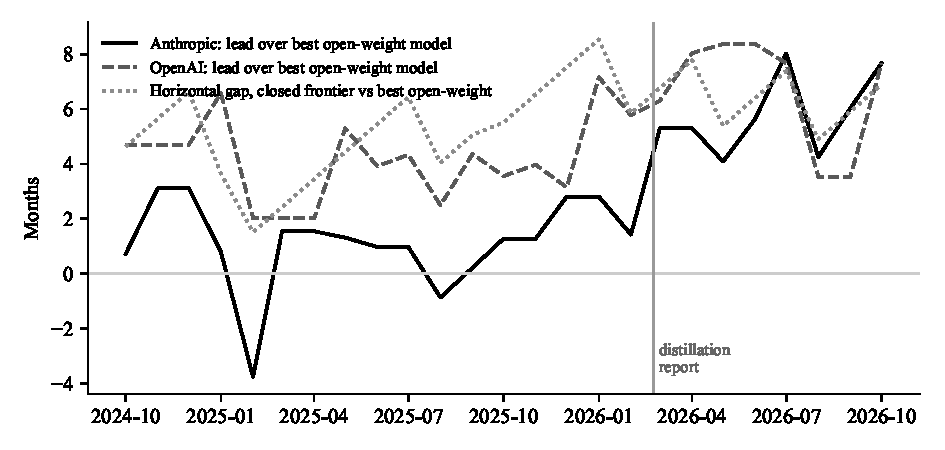
\includegraphics[width=\textwidth]{figures/fig1_leads.pdf}
\caption{Lead of Anthropic and OpenAI over the best open-weight model, equation~\eqref{eq:lead}, and the horizontal gap between the closed and open-weight frontiers, monthly. Source: Epoch Capabilities Index, author's calculations.}
\label{fig:leads}
\end{figure}

The distillation report of 23 February 2026 named DeepSeek, Moonshot and MiniMax and described countermeasures. If those measures slowed the named laboratories, their models released afterwards should lag the closed frontier by more, relative to other open-weight models. Table~\ref{tab:did} compares the lag of each open-weight model, the months between its release and the date the closed frontier first reached its ECI, before and after March 2026. Both groups' lags rose by about two months, and the difference-in-differences is $+0.1$ months with a standard error of 1.7, so its 95\% interval runs from about $-3.2$ to $+3.4$ months. The test is uninformative rather than negative, for four reasons: there are only 19 models from the named laboratories; there is no pre-trend check; models released in March--October 2026 were mostly trained before the countermeasures; and the control group may also distil. The lag here is averaged over all open-weight models, not only the best, so it is not the horizontal gap of Figure~\ref{fig:leads}.

\begin{table}[t]
\centering
\begin{threeparttable}
\caption{Lag of open-weight models behind the closed frontier, months}
\label{tab:did}
\small
\begin{tabular}{lccc}
\toprule
 & Mar 2025--Feb 2026 & Mar 2026--Oct 2026 & Change \\
\midrule
\tabinput{tables/did.tex}
\bottomrule
\end{tabular}
\begin{tablenotes}\footnotesize
\item Mean lag, number of models in parentheses. The lag of a model is the time between its release and the date at which the closed frontier first reached its ECI. The last row is the interaction coefficient from an OLS regression of the lag on group, period and their product, with heteroskedasticity-robust standard error.
\end{tablenotes}
\end{threeparttable}
\end{table}

\section{Pricing the lead}\label{sec:price}

\subsection{Hedonic regression}

I estimate
\begin{equation}
\log p_m = a + b\,\ECI_m + \gamma\,\mathrm{open}_m + \varepsilon_m
\label{eq:hedonic}
\end{equation}
on the 89 models released since July 2025, where $p_m$ is the blended price. The coefficient $b$ is the proportional price increase per ECI point and $\gamma$ the log price difference between open and closed weights at equal capability. Table~\ref{tab:hedonic} reports four specifications and Figure~\ref{fig:hedonic} the data.

\begin{table}[t]
\centering
\begin{threeparttable}
\caption{Hedonic regressions of API price on capability}
\label{tab:hedonic}
\small
\begin{tabular}{lcccccc}
\toprule
Specification & $b$ & $\gamma$ & $e^{\gamma}$ & $\lambda$, months & $N$ & $R^2$ \\
\midrule
\tabinput{tables/hedonic.tex}
\bottomrule
\end{tabular}
\begin{tablenotes}\footnotesize
\item Dependent variable: log blended price per million tokens, OpenRouter, 22 October 2026. Models released since July 2025. Heteroskedasticity-robust standard errors in parentheses. $\lambda = 1/(b v)$ with $v = 1.43$ ECI points per month. Vintage control: release date in years. A bootstrap of the baseline (2,000 draws) gives $\lambda$ = 6.9 [5.2; 11.0] and $e^{\gamma}$ = 0.38 [0.22; 0.61], 90\% intervals. Adding $\ECI \times \mathrm{open}$ gives an interaction of $-0.013$ (0.048).
\end{tablenotes}
\end{threeparttable}
\end{table}

In the baseline, a one-point increase in ECI raises price by about 10\%, and an open-weight model costs 0.37 times as much as a closed model of equal capability. The slopes for open and closed models are statistically indistinguishable, so the two price schedules are parallel in logs. Since the closed frontier advances $v$ points a month, a lead of $L$ months carries a price premium $e^{bvL} = e^{L/\lambda}$ with $\lambda = 1/(bv) = 6.9$ months. Controlling for release date raises $b$ and lowers $\lambda$ to 3.6 months, because newer models are cheaper at given capability; developer fixed effects give 7.7 months. Clustering standard errors by developer (13 clusters) raises the standard error of $b$ from 0.022 to 0.032. Section~\ref{sec:results} reports results for $\lambda$ = 3.6, 6.9 and 11.0.

The closed-weight premium can be compared with \citet{demirer2025market,demirer2026jep}, who report that open-source models cost about 90\% less than closed models of the same intelligence, a price ratio of about ten, against 2.6 here (bootstrap interval 1.6--4.5). The two measurements differ: they compare models within intelligence tiers in usage data from 2024--2025, while this paper uses list prices from a single October 2026 cross-section and a continuous capability index. For the valuation results the size of the premium does not matter. In the margin curve derived below only the product of the premium and a calibrated cost parameter enters, so replacing $e^{\gamma} = 0.38$ by 0.10 leaves every implied lead and value in Section~\ref{sec:results} unchanged. What matters is the slope $b$.

\begin{figure}[t]
\centering
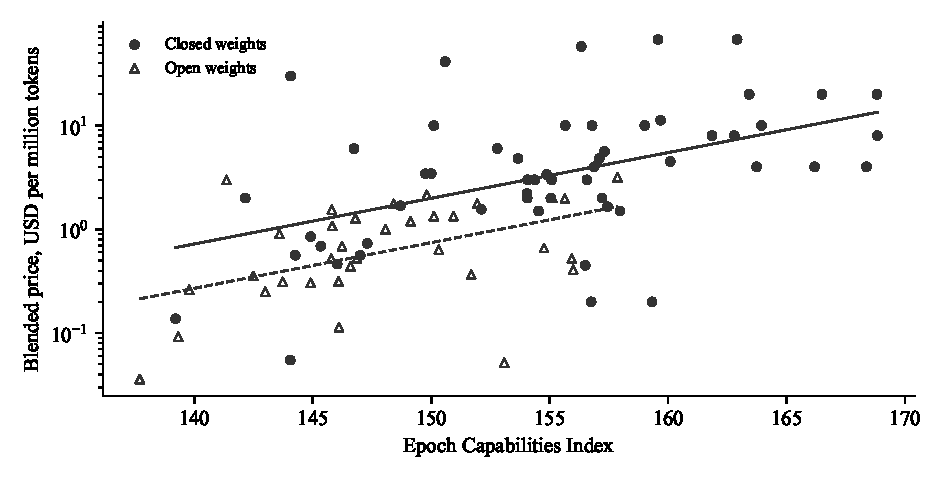
\includegraphics[width=\textwidth]{figures/fig2_hedonic.pdf}
\caption{Blended API price and capability, models released since July 2025, with baseline fit of equation~\eqref{eq:hedonic}. Sources: Epoch AI, OpenRouter.}
\label{fig:hedonic}
\end{figure}

Two caveats apply. Prices are per token, not per task, and reasoning models use more tokens per task. And list prices of older closed models are seldom revised, which tends to flatten the estimated slope; the vintage-controlled specification addresses this and gives a shorter $\lambda$.

\subsection{Cost or rent?}

The slope $b$ need not measure willingness to pay for a lead. More capable models are larger and cost more to serve, so price can rise with capability even in a competitive market. Open-weight models allow the two to be separated, because their price is close to the cost of serving them: their slope estimates the cost gradient, and the difference between the closed and open slopes estimates the part of the closed price that rises with capability faster than cost, which is the rent a lead can earn. Table~\ref{tab:decomp} reports both.

\begin{table}[t]
\centering
\begin{threeparttable}
\caption{Price slope in capability: cost and rent}
\label{tab:decomp}
\small
\begin{tabular}{lccccc}
\toprule
Slope & Estimate & Robust s.e. & Clust.\ s.e. & Bootstrap 90\% & $\lambda$, months \\
\midrule
\tabinput{tables/decomp.tex}
\bottomrule
\end{tabular}
\begin{tablenotes}\footnotesize
\item OLS of log blended price on ECI, an open-weight dummy and their interaction, 89 models released since July 2025. Clustered standard errors by developer (13 clusters). Bootstrap: 4,000 resamples of models. $\lambda = 1/(b v)$, $v = 1.43$.
\end{tablenotes}
\end{threeparttable}
\end{table}

The rent slope is 0.013 with a 90\% interval from $-0.065$ to 0.094, and in 40\% of bootstrap draws it is zero or negative. Its upper bound corresponds to $\lambda = 7.4$ months, close to the time constant implied by the whole slope; its point estimate corresponds to $\lambda = 54$ months, that is, almost no premium. A cross-section of list prices therefore cannot establish that the lead is priced. The analysis below uses the whole slope, $\lambda = 6.9$, which is the upper end of what the data allow, so that the value it attributes to the lead is an upper bound. Identifying the rent requires a different design, such as the change in a closed model's price when an open-weight model reaches its capability.

\subsection{From prices to a margin curve}

Suppose the frontier developer sells at a price equal to that of the best open-weight model, $p_O$, times the closed-weight premium $e^{-\gamma}$ and the lead premium $e^{L/\lambda}$, and that its serving cost is a multiple $\kappa$ of $p_O$, which is close to the open model's marginal cost. Then
\begin{equation}
GM(L) = 1 - \kappa\, e^{\gamma}\, e^{-L/\lambda}, \qquad \frac{dGM}{dL} = \frac{1 - GM}{\lambda}.
\label{eq:gm}
\end{equation}
The scale $\kappa$ cannot be estimated from prices. I calibrate it so that a closed developer with a six-month lead earns a long-run gross margin of 75\%, close to the 77\% that Anthropic was reported to target for 2028 \citep{techcrunch2025anthropic}; this gives $\kappa = 1.57$. The same curve is used for every closed developer, which places them on it according to their observed lead. It implies a gross margin of 40\% with no lead, 67\% with four months and 80\% with Anthropic's October 2026 lead of 7.7 months; at 75\% a month of lead is worth 3.6 percentage points of margin. The calibration point is open to an objection of timing: the 77\% target was reported in November 2025, when Anthropic's lead was only about 1.3 months, and at that lead the curve gives 51\%. Calibrating instead to 77\% at 1.3 months puts every closed developer with a lead of more than about four months at the margin cap, so that further lead is worth nothing; Section~\ref{sec:results} reports this case. For open-weight developers I set $e^{\gamma} = 1$, so that without a lead their margin is negative and they are valued as hosts of commodity models (below).

\section{Valuation model}\label{sec:model}

The model is a ten-year discounted cash flow with a Gordon terminal value; all parameters except revenue, cash and the lead are common to all firms. First-year revenue growth $g_0$ decays exponentially to 3\% with a time constant of 2.5 years, $g_i = 0.03 + (g_0 - 0.03)e^{-i/2.5}$. The gross margin moves from the reported level to $GM(L)$ over three years. Research and development spending falls from 45\% of revenue to 22\% with a time constant of 2.5 years; selling, general and administrative costs are 12\%; the tax rate is 21\%. Reinvestment in data centres and working capital is 25\% of the increase in revenue, and the terminal value assumes a return on new capital of 25\%. The discount rate is 12\%, with 10\% and 14\% as alternatives.

The lead affects value through margin and through revenue: a higher margin at given serving cost is a higher price, and demand responds with a price elasticity $\varepsilon$, so that revenue scales with $\bigl((1-GM(L_0))/(1-GM(L))\bigr)^{1-\varepsilon}$ relative to revenue at the observed lead $L_0$. The baseline is $\varepsilon = 1.1$, the short-run elasticity for individual models estimated by \citet{demirer2025market}. Two further arguments point the same way. A firm with pricing power sets price on the elastic part of its demand curve, and the Lerner condition $(p - c)/p = 1/\varepsilon$ with a 75\% margin gives $\varepsilon = 1.33$; and the demand for one developer's tokens is more elastic than the demand for tokens in general. With $\varepsilon > 1$ a higher price lowers revenue, so the lead raises value only through margin. I report $\varepsilon = 0.5$, which an earlier version of this paper used as the baseline, and $\varepsilon = 1.33$ as alternatives. A developer whose lead is too short to cover the cost of staying at the frontier can stop: it then becomes a host of its own models, with a gross margin of 25\% (the level of competitive open-weight hosts), research spending of 6\% of revenue and a 20\% loss of revenue. The model takes the better of the two strategies, and equity value cannot fall below cash.

For a valuation event with price $V$ the implied lead solves $\mathrm{DCF}(L; g_0) = V$. Holding the other parameters fixed, this defines a curve in the $(g_0, L)$ plane along which the price is justified. Two points on it are of particular interest: the growth rate that justifies the price if the lead stays at its observed value, and the lead that justifies the price if growth equals an independent forecast.

\section{Results}\label{sec:results}

\subsection{Iso-value curves}

Figure~\ref{fig:iso} shows the iso-value curves for four Anthropic and three OpenAI events. Each curve is steep and convex: between first-year growth of 150\% and 200\% the implied lead falls by a factor of two to three, and above 250\% it is close to zero. Each curve ends at the top where the margin reaches its cap of 85\%, at a lead of about 9.5 months: a price to the left of the curve's end cannot be justified at any lead, only by faster growth. Within the plausible range of growth, then, a valuation does not determine the lead it presumes; it determines the trade-off, and the range of growth over which the lead matters at all is narrow.

\begin{figure}[t]
\centering
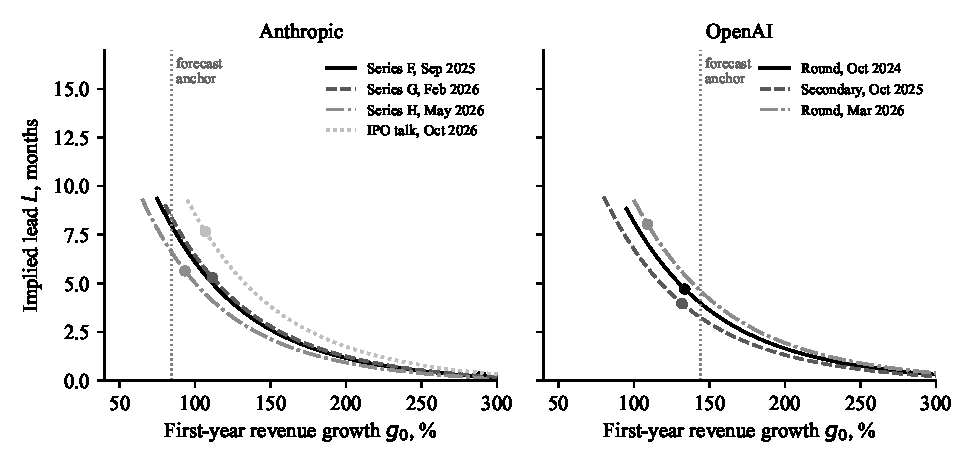
\includegraphics[width=\textwidth]{figures/fig3_iso.pdf}
\caption{Iso-value curves: combinations of first-year revenue growth and lead over the best open-weight model at which the discounted cash flow equals the valuation. Dots mark the observed lead at the event date. Vertical lines mark growth implied by independent revenue forecasts: for Anthropic, \$190--200 billion in 2028 from a run-rate of \$67 billion; for OpenAI, more than \$280 billion in 2030 from \$24 billion. Discount rate 12\%, long-run margin 75\% at a six-month lead, price elasticity of demand 1.1, $\lambda = 6.9$ (upper bound of the lead premium). Curves end where the margin reaches its cap.}
\label{fig:iso}
\end{figure}

The curves for Anthropic's three funding rounds lie close together despite a fivefold increase in valuation between September 2025 and May 2026, because revenue grew faster than price: the ratio of valuation to run-rate fell from 37 to 21. The October 2026 figure of \$2 trillion lies to the right of the May curve, so for a given lead it requires faster growth. The dots, which mark the observed lead, move up the curves over time as Anthropic's lead widened.

\subsection{Required growth at the observed lead}

Table~\ref{tab:events} reports, for every event, the first-year growth that justifies the price if the lead stays at its observed value. For the frontier developers in 2026 it lies between 93\% and 111\%; for Anthropic in 2025, when its lead was about one month, between 200\% and 290\%. Ex post, growth was much faster than that: Anthropic's run-rate rose about tenfold in the eleven months after March 2025 and about thirteenfold in the ten months after September 2025, and OpenAI's about 3.6-fold and fourfold in the twelve months after October 2024 and March 2025. Each of the four rounds for which a year of subsequent data exists was cheap in hindsight, although this is the comparison that survivorship would produce.

For developers without a lead the required growth is roughly 200--400\%. xAI, Mistral and Cohere are closed-weight developers whose best models are behind the open-weight frontier; Zhipu, MiniMax and Moonshot release open weights. In the model all of them earn either the margin of a closed developer with no lead or that of a commodity host, and their prices can be reached only through very fast growth.

\begin{table}[p]
\centering
\begin{threeparttable}
\caption{Valuation events, observed lead and required growth}
\label{tab:events}
\footnotesize
\setlength{\tabcolsep}{4pt}
\begin{tabular}{lllrrrrrl}
\toprule
Firm & Date & Event & Value, \$bn & Run-rate, \$bn & Multiple & $L$, months & $g_0$, \% & Conf. \\
\midrule
\tabinput{tables/events.tex}
\bottomrule
\end{tabular}
\begin{tablenotes}\footnotesize
\item Value: post-money valuation, or market value for listed firms and SpaceX's acquisition price for xAI; the October 2026 Anthropic figure is a reported offering valuation, not a transaction. Run-rate: annualised revenue nearest the event; some are interpolated (Appendix Table~\ref{tab:sources}). $L$: lead over the best open-weight model by equation~\eqref{eq:lead}; n/a where the developer has no ECI-scored model before the event. $g_0$: first-year revenue growth at which the discounted cash flow equals the value if the lead stays at $L$; discount rate 12\%.
\end{tablenotes}
\end{threeparttable}
\end{table}

\subsection{Anchoring on revenue forecasts}

Two events have an independent growth forecast. For Anthropic's offering, the revenue path of \$190--200 billion in 2028 that bankers were reported to use corresponds to $g_0 = 85\%$. For OpenAI's March 2026 round, the company's plan of more than \$280 billion in 2030 corresponds to $g_0 = 144\%$. Table~\ref{tab:anchored} reports the value at the observed lead, the implied lead and the value of one month of lead under four combinations of discount rate and long-run margin and two demand elasticities.

\begin{table}[t]
\centering
\begin{threeparttable}
\caption{Implied lead with growth anchored on revenue forecasts}
\label{tab:anchored}
\small
\begin{tabular}{cccccccc}
\toprule
 & & \multicolumn{3}{c}{Anthropic, \$2,000bn, Oct 2026} & \multicolumn{3}{c}{OpenAI, \$852bn, Mar 2026} \\
\cmidrule(lr){3-5}\cmidrule(lr){6-8}
Discount & $GM$ at & DCF at & Implied & Month of & DCF at & Implied & Month of \\
rate & 6 months & $L$, \$tn & $L$ & lead, \% & $L$, \$tn & $L$ & lead, \% \\
\midrule
\tabinput{tables/anchored.tex}
\bottomrule
\end{tabular}
\begin{tablenotes}\footnotesize
\item Observed lead: Anthropic 7.7 months, OpenAI 8.0. ``Month of lead'': change in value from one more month of lead, central difference, as a share of value at the observed lead. With a long-run margin of 85\% the margin cap is raised from 85\% to 92\%. ``Unattainable'': the price exceeds the value at any lead; 0.0: the price is justified even without a lead. Upper panel: price elasticity of demand 1.1 (baseline, following \citet{demirer2025market}); lower panel: 0.5.
\end{tablenotes}
\end{threeparttable}
\end{table}

In the baseline (upper panel, 12\% discount rate, 75\% margin) Anthropic is worth \$1.36 trillion if its lead stays at 7.7 months. The value rises with the lead only until the margin cap is reached, at about 9.8 months and \$1.47 trillion, so \$2 trillion cannot be reached at any lead; with a 10\% discount rate the maximum is \$1.97 trillion. Only with a 10\% discount rate and an 85\% long-run margin does the price become attainable, at a lead of 5.0 months. On the bankers' revenue path the offering price therefore presumes faster growth, not a particular lead. If the lead instead returned to its January 2025--October 2026 median of 1.5 months, the model gives \$512 billion, and averaging over the monthly leads observed in that period gives \$716 billion (at 10\%: \$701 billion and \$967 billion).

OpenAI's March 2026 price was below the value at its observed lead of 8.0 months in every combination, \$1.43--2.25 trillion, and implied a lead of 0--2.9 months in the upper panel and 0.7--4.6 months in the lower. The round, in other words, priced in substantial erosion of the lead; Figure~\ref{fig:leads} shows that OpenAI's lead did fall to 3.5 months by August before recovering.

A month of lead is worth 2--5\% of value in the upper panel and 10--13\% in the lower. With elastic demand a higher price brings no extra revenue, so the lead raises value only through margin; and because the elasticity of margin with respect to the lead is $(1-GM)/\lambda$, it is smaller when the margin is already close to its ceiling.

\subsection{Sensitivity}

Table~\ref{tab:sens} varies one assumption at a time from the baseline: the decay of the lead premium, including the rent-only point estimate of Section~\ref{sec:price}; the demand elasticity; the margin cap; the calibration of the margin curve, including the chronologically consistent anchor of 77\% at a 1.3-month lead; the growth anchors, by $\pm 20\%$ of the forecast revenue; and reinvestment, which at 25\% of new revenue is low for firms that report compute commitments of more than \$600 billion.

\begin{table}[t]
\centering
\begin{threeparttable}
\caption{Sensitivity of the anchored results}
\label{tab:sens}
\footnotesize
\setlength{\tabcolsep}{4pt}
\begin{tabular}{lcccccc}
\toprule
 & \multicolumn{3}{c}{Anthropic, \$2,000bn, Oct 2026} & \multicolumn{3}{c}{OpenAI, \$852bn, Mar 2026} \\
\cmidrule(lr){2-4}\cmidrule(lr){5-7}
Specification & DCF, \$tn & Impl.\ $L$ & Month, \% & DCF, \$tn & Impl.\ $L$ & Month, \% \\
\midrule
\tabinput{tables/sensitivity.tex}
\bottomrule
\end{tabular}
\begin{tablenotes}\footnotesize
\item Baseline: discount rate 12\%, $\lambda = 6.9$, $\varepsilon = 1.1$, margin 75\% at a six-month lead, cap 85\%, growth anchors as in Table~\ref{tab:anchored}, reinvestment 25\% of new revenue. Each row changes one assumption. DCF: value at the observed lead. ``unatt.'': the price exceeds the value at any lead. ``Month'': value of one more month of lead as a share of value at the observed lead (Anthropic 7.7 months, OpenAI 8.0).
\end{tablenotes}
\end{threeparttable}
\end{table}

Two results hold in every row. Anthropic's \$2 trillion is unattainable on the bankers' revenue path in thirteen of fourteen specifications; only 20\% more revenue in 2028 brings it within reach, at a lead of 8.6 months. And OpenAI's March 2026 price implies a lead of 0--5.4 months in every specification, below the lower end of the 90\% interval of its measured lead, 6.6--10.5 months (Table~\ref{tab:leadci}). The value of a month of lead does not hold: it ranges from zero, when the margin curve is calibrated to the 2025 lead or the premium is the rent-only point estimate, to 10\% with a lower margin anchor and 13\% with inelastic demand. Higher reinvestment lowers the value at the observed lead by up to a fifth and raises the lead OpenAI's price implied, but changes neither conclusion. Because the baseline uses the upper bound of the lead premium that the baseline regression allows, these values of the lead are, if anything, overstated.

\subsection{Developers without a lead}

For the developers that have no lead, Figure~\ref{fig:gm} reports the alternative inversion: the constant long-run gross margin that justifies the price, as a function of first-year growth, ignoring the lead. Zhipu's October 2026 market value requires a margin of 69\% at 100\% growth and 45\% at 200\%; MiniMax's, 78\% and 47\%. They reported 26\% and 18\% for the first half of 2026. Below roughly 40\% no positive valuation is possible under the common cost structure, so the curves flatten there. Moonshot and Mistral, whose valuations are higher relative to revenue, require more. These prices therefore embed either a change in the cost structure, a margin these firms have not yet earned, or a value that a cash flow model does not capture, such as strategic or national-security considerations.

\begin{figure}[t]
\centering
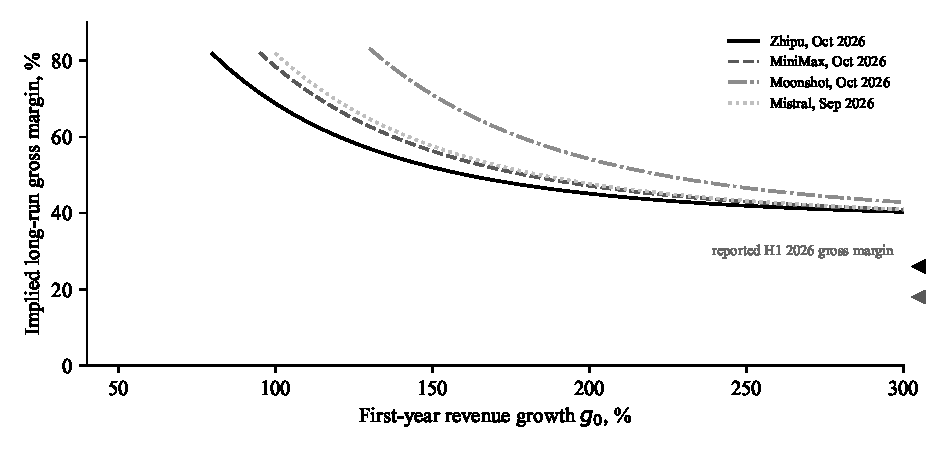
\includegraphics[width=\textwidth]{figures/fig4_gm.pdf}
\caption{Constant long-run gross margin at which the discounted cash flow equals the valuation, developers without a lead. Arrows: reported gross margin, first half of 2026 (Zhipu 26\%, MiniMax 18\%). Discount rate 12\%.}
\label{fig:gm}
\end{figure}

\section{Limitations}\label{sec:limits}

The margin curve rests on prices of tokens and on an assumption about serving cost. Whether the lead earns any premium is not identified by the cross-section of prices (Table~\ref{tab:decomp}); the analysis uses the upper bound. The time constant $\lambda$ changes by a factor of two across specifications. The scale $\kappa$ is calibrated, not estimated, its calibration point is in tension with the timing of the lead, and Anthropic's reported gross margin is not defined consistently across sources. The value of a month of lead depends heavily on the price elasticity of demand, which is not estimated here.

The lead is a constant in the valuation model: it does not decay, and distillation, which would shorten it, does not enter the model. A version in which the lead shrinks at a rate set by imitation would turn the competitive advantage period into a duration in the sense of \citet{mauboussin1997cap}, rather than a level that persists into the terminal value. Competition among closed developers is also ignored: Anthropic and OpenAI, with similar leads over open-weight models, receive the same margin, although two leaders compete each other's rents down.

The valuation model is deliberately simple and common to all firms, including the Hong Kong-listed ones. Its cost parameters are not taken from filings, growth is deterministic, and the skewed distribution of outcomes that drives venture valuations is absent, so the conclusions about developers without a lead describe what the template requires rather than diagnose the market. Firm-specific growth paths, revenue concentration (about 20\% of Anthropic's first-half 2026 revenue reportedly came from two customers), compute commitments of more than \$600 billion, only partly reflected in the reinvestment sensitivity, and dilution from convertible instruments are not modelled. The implied lead absorbs every such omission, in the same way that implied volatility absorbs every departure from the Black--Scholes assumptions; its level should be read accordingly, and the iso-value curves, which display the dependence on growth explicitly, are the more robust object.

Several valuation inputs come from press reports rather than filings, and two are interpolated run-rates. The private-round valuations are post-money prices of preferred stock with protective terms, which overstate the value of common equity. The sample of events with independent growth forecasts has two members, and the Anthropic forecast comes from the banks marketing the offering. Anthropic's public registration statement, if it is filed in November 2026 as reported, and subsequent analyst forecasts should add both reliable fundamentals and more anchors.

\section{Conclusion}

Valuation practice infers a competitive advantage period from prices; in frontier AI the corresponding lead over imitators can also be measured, almost monthly, though with intervals of several months. Whether that lead is priced is harder to say than it looks: a cross-section of API prices rises with capability at the same rate for open-weight models, sold near cost, as for closed ones, so it cannot separate a leader's rent from the cost of serving larger models. Using the most favourable reading of the prices, the iso-value curves of growth against implied lead show that the valuations of 2025--2026 do not identify the lead they presume without a view on growth. With the growth forecasts that are available, two conclusions survive every specification tried: on its bankers' revenue path, a \$2 trillion valuation of Anthropic cannot be justified at any lead and presumes faster growth, and OpenAI's last private round presumed that its lead would narrow. The value of a month of lead, which an earlier version of this paper put at 10--13\% of firm value, is not robust: it ranges from zero to about a tenth and is about 5\% in the baseline. Developers without a lead are priced on growth far beyond what a deterministic cash flow model can support. Whether distillation shortens leads remains open: the laboratories that Anthropic accused of distillation fell behind no faster and no slower than other open-weight developers after its countermeasures, but the test cannot rule out effects of up to three months.

\section*{Declarations}
\noindent\textit{Use of AI tools.} Data collection, code and drafting were assisted by Claude, a large language model developed by Anthropic, one of the firms studied. The author reviewed all results and is responsible for the content.

\noindent\textit{Conflicts of interest.} The author has no financial or professional relationship with any of the firms studied.

\noindent\textit{Data availability.} Epoch AI data are available under CC BY 4.0; OpenRouter prices from its public API. Code, the valuation panel, the Epoch snapshot used and derived data are available at \url{https://github.com/veshidar-dot/anthropic-openai-valuation-distillation}.

\begin{thebibliography}{99}
\setlength{\itemsep}{2pt}
\small

\bibitem[Andrews and Farboodi(2026)]{andrews2026markets}
Andrews, I., and Farboodi, M. (2026). Do markets believe in transformative AI? Working paper, Massachusetts Institute of Technology, version of July 2026. \url{https://economics.mit.edu/}.

\bibitem[Anthropic(2026)]{anthropic2026distill}
Anthropic (2026). Detecting and preventing distillation attacks. Company announcement, 23 February 2026. \url{https://www.anthropic.com/news}.

\bibitem[Berk et~al.(2004)Berk, Green, and Naik]{berk2004valuation}
Berk, J.~B., Green, R.~C., and Naik, V. (2004). Valuation and return dynamics of new ventures. \textit{Review of Financial Studies}, 17(1), 1--35.

\bibitem[Bj\"orkegren(2025)]{bjorkegren2025open}
Bj\"orkegren, D. (2025). Market beliefs about open vs.\ closed AI. arXiv:2512.14969 [econ.GN], version 3, 26 January 2026.

\bibitem[Damodaran(2009)]{damodaran2009young}
Damodaran, A. (2009). Valuing young, start-up and growth companies: estimation issues and valuation challenges. Working paper, Stern School of Business, New York University. SSRN 1418687.

\bibitem[Demirer et~al.(2025)Demirer, Fradkin, Tadelis, and Peng]{demirer2025market}
Demirer, M., Fradkin, A., Tadelis, N., and Peng, S. (2025). The emerging market for intelligence: pricing, supply, and demand for LLMs. NBER Working Paper 34608, December 2025.

\bibitem[Demirer et~al.(2026)Demirer, Fradkin, and Tadelis]{demirer2026jep}
Demirer, M., Fradkin, A., and Tadelis, N. (2026). The emerging market for intelligence: how firms buy and sell AI. \textit{Journal of Economic Perspectives}, 40(3), 23--46.

\bibitem[Epoch AI(2026a)]{epoch2026benchmarks}
Epoch AI (2026a). Capabilities and benchmarking. Data hub, retrieved 22 October 2026. \url{https://epoch.ai/benchmarks}.

\bibitem[Epoch AI(2026b)]{epoch2026gap}
Epoch AI (2026b). Data insight on the capability gap between open-weight and closed models, 29 May 2026. \url{https://epoch.ai/data-insights/open-closed-eci-gap}.

\bibitem[Hinton et~al.(2015)Hinton, Vinyals, and Dean]{hinton2015distilling}
Hinton, G., Vinyals, O., and Dean, J. (2015). Distilling the knowledge in a neural network. arXiv:1503.02531.

\bibitem[Kogan et~al.(2017)Kogan, Papanikolaou, Seru, and Stoffman]{kogan2017innovation}
Kogan, L., Papanikolaou, D., Seru, A., and Stoffman, N. (2017). Technological innovation, resource allocation, and growth. \textit{Quarterly Journal of Economics}, 132(2), 665--712.

\bibitem[Mansfield(1985)]{mansfield1985leak}
Mansfield, E. (1985). How rapidly does new industrial technology leak out? \textit{Journal of Industrial Economics}, 34(2), 217--223.

\bibitem[Mansfield et~al.(1981)Mansfield, Schwartz, and Wagner]{mansfield1981imitation}
Mansfield, E., Schwartz, M., and Wagner, S. (1981). Imitation costs and patents: an empirical study. \textit{Economic Journal}, 91(364), 907--918.

\bibitem[Mauboussin and Johnson(1997)]{mauboussin1997cap}
Mauboussin, M., and Johnson, P. (1997). Competitive advantage period: the neglected value driver. \textit{Financial Management}, 26(2), Summer 1997.

\bibitem[OpenRouter(2026)]{openrouter2026}
OpenRouter (2026). Models API, \texttt{GET /api/v1/models}. Retrieved 22 October 2026. \url{https://openrouter.ai/api/v1/models}.

\bibitem[P\'astor and Veronesi(2006)]{pastor2006nasdaq}
P\'astor, \v{L}., and Veronesi, P. (2006). Was there a Nasdaq bubble in the late 1990s? \textit{Journal of Financial Economics}, 81(1), 61--100.

\bibitem[P\'astor and Veronesi(2009)]{pastor2009revolutions}
P\'astor, \v{L}., and Veronesi, P. (2009). Technological revolutions and stock prices. \textit{American Economic Review}, 99(4), 1451--1483.

\bibitem[Rappaport and Mauboussin(2001)]{rappaport2001expectations}
Rappaport, A., and Mauboussin, M.~J. (2001). \textit{Expectations Investing: Reading Stock Prices for Better Returns}. Boston: Harvard Business School Press.

\bibitem[Rosen(1974)]{rosen1974hedonic}
Rosen, S. (1974). Hedonic prices and implicit markets: product differentiation in pure competition. \textit{Journal of Political Economy}, 82(1), 34--55.

\bibitem[Schwartz and Moon(2000)]{schwartz2000internet}
Schwartz, E.~S., and Moon, M. (2000). Rational pricing of internet companies. \textit{Financial Analysts Journal}, 56(3), 62--75.

\bibitem[TechCrunch(2025)]{techcrunch2025anthropic}
TechCrunch (2025). Anthropic expects B2B demand to boost revenue to \$70B in 2028: report. 4 November 2025. \url{https://techcrunch.com/2025/11/04/anthropic-expects-b2b-demand-to-boost-revenue-to-70b-in-2028-report/}.

\end{thebibliography}

\appendix
\section{Sources of the valuation panel}

\begingroup
\footnotesize
\setlength{\tabcolsep}{4pt}
\begin{longtable}{lll>{\raggedright\arraybackslash}p{0.56\textwidth}}
\caption{Sources for Table~\ref{tab:events}}\label{tab:sources}\\
\toprule
Firm & Date & Event & Source and notes \\
\midrule
\endfirsthead
\toprule
Firm & Date & Event & Source and notes \\
\midrule
\endhead
\tabinput{tables/sources.tex}
\bottomrule
\end{longtable}
\endgroup

\end{document}
